% !TEX root = ../../math6370.tex
\newpage
\section{The Ring of Integers}
\subsection{Number Fields}

Algebraic Number Theory studies the arithmetic of number fields --- the ring of integers of number fields and their ideals, units, and factorizations. Number theoretic questions are then posed in terms of these algebraic objects and their properties. To begin, we recall the definition of the basic object of study in Algebraic Number Theory --- number fields. 


\begin{dfn}[Number Field]
A number field $K$ is a finite extension of $\Q$, i.e. a finite dimensional $\Q$-vector space. We can denote this pictorially as in the figure below. 
	\[
	\begin{tikzcd}
	K \arrow[dash]{d}{[K\,:\,\Q]=\,\dim_\Q K} \\
	\Q
	\end{tikzcd}
	\]
\end{dfn}


\begin{ex}[Number Fields] \label{ex:number_fields} \hfill
	\begin{enumerate}[(i)]
	\item The fields $\Q$, $\Q(\sqrt{2})$, $\Q(\sqrt[3]{2})$ are all number fields. These have dimension (as $\Q$-vector spaces) of 1, 2, and 3, respectively. 
	\item The cyclotomic fields: $\Q(\zeta_n)$, where $\zeta_n$ is a primitive $n$th root of unity.
	\item The field $\Q(\alpha)$, where $\alpha$ is a root of $x^3+2x^2+1$. \xqed \pskip
	\end{enumerate}
\end{ex}


Recall that a simple extension of a field $K$, say $L$, is an extension of the form $L= K(\alpha)$, where $\alpha$ is the root of some polynomial $p_\alpha(x) \in K[x]$. The examples of number fields in Example~\ref{ex:number_fields} are all simple extensions of $\Q$. These were not arbitrarily contrived `simple' examples of number fields. In fact, every number field arises in this way. Recall the following terminology: given a field extension $E/F$, an element $\alpha \in E$ is called a primitive element for $E/F$ if $E=F(\alpha)$. Then our preceding claim is that every number field possess a primitive element, which the following theorem justifies. 


\begin{thm}[Primitive Element Theorem] \label{thm:primelmthm}
If $K$ is a number field, then $K=\Q(\alpha)$, where $\alpha$ is the root of some polynomial $p_\alpha(x) \in \Q[x]$. 
\end{thm}

\pf See \cite[Ch. 14.4, Thm 25]{dummit}. Though there are proofs which avoid Galois Theory. For instance, the  proof of van der Waerden avoid Galois Theory and is `constructive.' This is essentially the proof given in \cite{murty}, but can also be found more thoroughly written out in \cite{brown}. \qed \pskip


Generally, if $E/F$ is a separable extension of finite degree, then $E=F(\alpha)$ for some $\alpha \in E$. Of course, the definition of a number field excludes infinite extensions of $\Q$ such as $\R$, $\C$, and $\Q(\{\sqrt[n]{2} \colon n \in \N\})$. Of course, there are even examples of infinite extensions of $\Q$ when the extension is simple, e.g. $K=\Q(e)$ or $K=\Q(\pi)$. But remember, the term `number field' will always refer to finite extensions of $\Q$. 


The traditional object of interest in number theory is $\Z \subseteq \Q$. What is `interesting' about $\Z$, among other things, is factorization. Of course, there is no factorization in $\Q$ because $\Q$ is a field. Of course, fields are `nicer' to work with. But constructing number fields, what should be the analog for a general number field $K$, i.e. what should the object $\O \subseteq K$ be so that factoring is `interesting'. What are the `integers' for a number field? The first goal for this course will be to define such an object and to study its properties. 


	\[
	\begin{tikzcd}
	? \arrow[dash]{r} & K \arrow[dash]{d}{[K \colon \Q]} \\
	\Z \arrow[dash]{r} & \Q
	\end{tikzcd}
	\]



% -------------------
% Ring of Integers
% -------------------
\subsection{The Ring of Integers}


Let $K$ be a number field. Choose $\alpha \in K$ and let $n=[K:\Q]$. Let $\phi: \Q[x] \to K$ be the homomorphism of $\Q$-algebras given by $x \mapsto \alpha$. This map is not injective (it is a map of an infinite dimensional vector space to a finite dimensional vector space). Therefore, the kernel is nonzero. The ring $\Q[x]$ is a PID so that the $\ker \phi$ is nonzero and principal. This induces an isomorphism $\widetilde{\phi}: \Q[x]/(p_\alpha(x)) \to K$, where $p_\alpha(x)$ is the minimal monic irreducible polynomial in $\Q[x]$ with $\alpha$ as a root (its so-called minimal polynomial). Denote by $\Q[\alpha]$ the image of $\widetilde{\phi}$ in $K$, i.e. the $\Q$-algebra generated by $\alpha$. Because $p_\alpha(x)$ is irreducible, $(p_\alpha(x))$ is maximal and hence $\Q[x]/(p_\alpha(x))$ is a field. But because $\Q[\alpha] \cong \Q[x]/(p_\alpha(x))$, we must have $\Q[\alpha] \cong \Q(\alpha)$ so that $\Q[\alpha]$ is a field. Note that since $\Q \subseteq K$, certainly $\Z \subsetneq K$. 


Now recall that $\alpha \in K/\Q$ is an algebraic number if $p_\alpha(x) \in \Q[x]$. [Such a $p_\alpha(x)$ exists because we cannot have $\alpha$ transcendental since we assume that $K$ is a number field.] So if $\alpha$ is an algebraic number, then the work in the preceding paragraph shows that $\Q[\alpha] \cong \Q(\alpha)$. Using this isomorphism, we shall often, by abuse of notation, treat $\Q[\alpha] = \Q(\alpha)$. We are interested in a very special type of algebraic number. 


\begin{dfn}[Algebraic Integer]
Let $K/\Q$ be a number field. We say $\alpha \in K$ is an algebraic integer if $p_\alpha(x)$ has coefficients in $\Z$, i.e. $p_\alpha(x) \in \Z[x]$. 
\end{dfn}


This definition allows us to define a candidate for a subring of $K$ where factorization will be `interesting.' 


\begin{dfn}[Ring of Integers]
Let $K/\Q$ be a number field. Define the ring of integers of  $K$, denoted $\O_K$, to be the set of algebraic integers of $K$. This is also sometimes denoted $\Z_K$. 
\end{dfn}


Despite being part of the definition, it is not immediately clear that $\O_K$ is even a ring. We shall prove this later. We will first look at some examples of rings of integers. The first example will show that this definition of `rings of integers' does reproduce the literal ring of integers $\Z$ in the case where $K= \Q$. [Note that because $p_r(x)= x - r \in \Z[x]$ for all $r \in \Z$, we always have $\Z \subseteq \O_K$.]


\begin{ex}\label{ex:zinq}
Take $K= \Q$. If $\alpha \in \Q$, then its minimal polynomial is $p_\alpha(x)= x - \alpha$. Now $p_\alpha(x) \in \Z[x]$ if and only if $\alpha \in \Z$. Therefore, $\O_\Q= \Z$. Then our definition of the ring of integers does indeed reproduce the motivating example of $\Z \subseteq \Q$. \xqed \pskip
\end{ex}


\begin{ex}
Take $K=\Q(\sqrt{-2})= \{ a + b \sqrt{-2} \colon a,b \in \Q \} \subseteq \C$ and $\alpha= a + b\sqrt{-2} \in K$. We have two cases: \pskip

\noindent $b=0$: If $b=0$, then $a \in \Q$. But then by the work in Example~\ref{ex:zinq}, $\alpha \in \O_K$ if and only if $\alpha \in \Z$. \pskip

\noindent $b\neq 0$: If $b \neq 0$,  then $p_\alpha(x)$ factors as 
	\[
	p_\alpha(x)=(x-(a+b\sqrt{-2}))(x-(a-b\sqrt{-2}))=x^2-2ax+(a^2+2b^2).
	\]
Therefore, $\alpha \in \O_K$ if and only if $2a \in \Z$ and $a^2+2b^2 \in \Z$. Let $N= a^2 + 2b^2$. Because $2a \in \Z$, we have $a= \frac{r}{2}$ for some $r \in \Z$. Then we have $N= a^2 + 2b^2= \frac{r^2}{4} + 2b^2$. But then clearing denominators shows $r^2 + 8b^2= 4N$, which implies that $r$ cannot be odd. Therefore, $r= 2k$ for some $k \in \Z$, which shows that $a= \frac{r}{2}= \frac{2k}{2}= k \in \Z$. 

But then $2b^2= N - a^2 \in \Z$ so that $2b^2= s$ for some $s \in \Z$. Using the fact that $b \in \Q$, write $b= \frac{u}{v}$ and $\gcd(u, v)= 1$. Then we have $2u^2= sv^2$. If $p$ is a prime dividing $v$, then $p^2 \mid (sv^2)= 2u^2$. Because $\gcd(u,v)=1$, we must have $p^2 \mid 2$, which is impossible because $2$ is not a square in $\Z$. Therefore, no prime divides $v$ so that $v= \pm 1$. But then $b^2= \frac{u^2}{v^2}= u^2$, forcing $b= \pm u \in \Z$. Therefore, we must have $a, b \in \Z$. \pskip
	
This shows that $\O_K= \Z[\sqrt{-2}]= \{ a + b \sqrt{-2} \colon a,b \in \Z \}$. Furthermore, one can show $\Z[\sqrt{-2}]$ is a UFD, i.e. factorial. \xqed \pskip
\end{ex}


There is one important motivating question we have not yet addressed: why do we care about `integers' in number fields rather than just considering the ordinary integers in $\Q \subseteq K$. The answer is simple: factorizations. In these larger rings, we might have `larger' and more `interesting' factorizations that we could use to solve problems that are otherwise more difficult than over $\Z$. 


\begin{ex}\label{ex:z(-sqrt(2))}
Find all solutions $x,y \in \Z$ for $y^2=x^3-2$. After a bit of experimentation, one can see that $(3,\pm 5)$ is a solution. However, are these the only solutions? Are there infinitely many integer solutions? We choose to work in $\Z[\sqrt{-2}]$ for the `extra factorizations' that it offers. Note that we shall use the fact that $\Z[\sqrt{-2}]$ is a UFD and $\Z[\sqrt{-2}]^\times=\{\pm 1\}$ without proof. [The latter will be easily proven using norms later, while the first fact follows from the fact that $\Z[\sqrt{-2}]$ is a Euclidean domain using the same canonical proof that $\Z[i]$ is Euclidean. All Euclidean domains are PIDs which are in turn UFDs.]

In $\Z[\sqrt{-2}]$, we have the factorization 
	\[
	x^3=y^2+2=(y+\sqrt{-2})(y-\sqrt{-2}). 
	\]
Write $x=u_1 \pi_1^{e_1}\cdots \pi_r^{e_r}$, where each $\pi_i$ is irreducible, $e_i \geq 1$, and $\pi_i \neq \pm \pi_j$ for $i \neq j$. Then we have
	\[
	u_1^3 \pi_1^{3e_1}\cdots \pi_r^{3e_r}=(y+\sqrt{-2})(y-\sqrt{-2}). 
	\]
We claim that $y+\sqrt{-2}$ and $y-\sqrt{-2}$ are relatively prime: choose an irreducible dividing both, say $\pi$. Then $\pi \mid \big(( y + \sqrt{-2}) - (y - \sqrt{-2}) \big)= 2\sqrt{-2}= (\sqrt{-2})^3$. By unique factorization in $\Z[\sqrt{-2}]$, up to a unit $u$, we must have $\pi= u\sqrt{-2}$. But the only units in $\Z[\sqrt{-2}]$ are $\{\pm 1\}$. Because $\pi^3= (\sqrt{-2})^3$, we must have $\pi= \sqrt{-2}$. Now as $\pi \mid (y + \sqrt{-2})$, we have $y + \sqrt{-2} = \pi (a + b \sqrt{-2})= \sqrt{-2} (a + b\sqrt{-2})= -2b + a\sqrt{-2}$ for some $a, b \in \Z$. But then as $\pi \mid (y + \sqrt{-2})$, we have $y + \sqrt{-2}= \sqrt{-2}(a + b\sqrt{-2})= -2b + a\sqrt{-2}$ for some $a, b \in \Z$. Therefore, $y= -2b$, which implies $x^3= y^2 + 2= 4b^2+2 \equiv 2 \mod 4$, a contradiction as no cube has residue 2 mod 4. This shows that $y + \sqrt{-2}$ and $y - \sqrt{-2}$ are relatively prime.

Then $\pi_i^{3e_i}$ divides $y+\sqrt{-2}$ or $y-\sqrt{-2}$ (but not both) for each $1 \leq i \leq r$. Then $y+\sqrt{-2}= u \prod_{i \in \I} \pi_i^{3e_i}$ for some $\I \subseteq \{ 1, \ldots, r \}$ and $u \in \Z[\sqrt{-2}]^\times= \{ \pm 1 \}$. This implies 
	\[
	y + \sqrt{-2}= u \prod_{i \in \I} \pi_i^{3e_i}= \prod_{i \in \I} \pi_i^{3e_i}= \left( \prod_{i \in \I} \pi_i^{e_i} \right)^3= (a + b\sqrt{-2} )^3
	\]
 for some $a,b \in \Z$. Expanding yields, $y+\sqrt{-2}=(a^3-6ab^2)+(3a^2b-2b^3)\sqrt{-2}$. This forces $y= a^3 - 6ab^2$ and $1= 3a^2b - 2b^3= b(3a^2 - 2b^2)$.

We now have a restriction on the possibilities for $y$! This restriction that would not have been as easily obtained working only in $\Z$. Now as $b (3a^2 - 2b^2)= 1$ with $a, b \in \Z$, it must be that $b \in \{\pm 1\}$. If $b= 1$, we have $3a^2 - 2= 1$, which gives $a= \pm 1$. Using $a= \pm 1$ and $b=1$, we have solutions $(3, \pm 5)$. If $b= -1$, then $3a^2(-1)-2(-1)^3=1$, which implies $3a^2=1$, a contradiction to the irrationality of $\sqrt{3}$. Therefore, the only integer solutions to $y^2= x^2 + 3$ are $(3, \pm 5)$. This also shows that this equation has only finitely many rational solutions.\footnote{On the other hand, there are infinitely many \emph{rational solutions} to this equation. In fact, this is an elliptic curve defined over $\Q$ with rank 1.} \xqed \pskip
\end{ex}


One must take care when using the factorization approach of Example~\ref{ex:z(-sqrt(2))}. Consider the following (non-)example. 


\begin{nex}\label{ex:factornonex}
Find all $(x,y) \in \Z^2$ satsifying $y^2=x^3-61$. Using the factorization in $\Z[\sqrt{-61}]$, we have $x^3=y^2+61=(y+\sqrt{-61})(y-\sqrt{-61})$. Using the method of Example~\ref{ex:z(-sqrt(2))}, one can show that there are no such solutions. But $(5, \pm 8)$ are both clearly solutions! \xqed \pskip
\end{nex}


The problem in Example~\ref{ex:factornonex} is that $\Z[\sqrt{-61}]$ is not a UFD: $5^3=8^2+61=(8+\sqrt{-61})(8-\sqrt{-61})$, where $5$, $(8+\sqrt{-61})$, and $(8-\sqrt{-61})$ are all irreducible in $\Z[\sqrt{-61}]$. Thus, Example~\ref{ex:z(-sqrt(2))} and Non-Example~\ref{ex:factornonex} show that not just factorization but \emph{unique} factorization is essential.  How does one cope with loss of unique factorization? Kummer (in approximately 1846) said there should be a further factorization into ``ideal numbers'' in order to recover unique factorization. This lead Dedekind to define ideals of a ring. He later gave the correct notion of factorization instead using (prime) ideals rather than factorization with elements. We shall see that while elements may/may not factor uniquely in $\O_K$, every ideal of $\O_K$ factors uniquely as a product of prime ideals. So we shall see that in Non-Example~\ref{ex:factornonex}, while elements $5$, $8 + \sqrt{-61}$, and $8 - \sqrt{-61}$ may not factor uniquely into irreducible, the ideals generated by these elements will factor uniquely into a product of prime ideals $\p, \q$:
	\[
	(5)= \p \q, \quad (8 + \sqrt{-61})= \p^3, \quad (8 - \sqrt{-61})= \q^3. 
	\]


To work towards this longterm goal, we want to study the properties of $\O_K$ further. As a short list of intermediate goals, we want to\dots
	\begin{itemize}
	\item Show $\O_K$ is a ring.
	\item Study the structure of abelian group $(\O_K, +)$ and show $\O_K \cong \Z^{[K:\Q]}$.
	\item Study the structure of units $\O_K^\times$.
	\item Show $\O_K$ has unique factorization into prime ideals.
	\item Measure failure of unique factorization, leading to the class group.
	\item Study the primes of $\O_K$ and how these primes `split'. 
	\end{itemize}


We shall begin by showing that $\O_K$ is a ring. The proof, which will be rather simple, will make use of some extra facts about algebraic integers.


\begin{prop}\label{prop:algint}
If $\alpha \in K$ is an algebraic integer, then the following are equivalent:
	\begin{enumerate}[(i)]
	\item $p_\alpha(x) \in \Z[x]$
	\item $f(\alpha)= 0$ for some monic polynomial $f(x) \in \Z[x]$
	\item $\Z[\alpha]$ is a finitely generated $\Z$-module
	\item there exists a nonzero finitely generated subgroup $M \subseteq K$ such that $\alpha M  \subseteq M$
	\end{enumerate}
\end{prop}

\pf We prove (i)$\iff$(ii) $\Rightarrow$ (iii) $\Rightarrow$ (iv) $\Rightarrow$ (i). 
\begin{enumerate}
\item[(i)$\to$(ii):] This is immediate.

\item[(ii)$\to$(iii):] If $f(x)=x^n + a_1x^{n-1} + \cdots + a_n$ has $\alpha$ as a root, then we can express the numbers $\{\alpha^i\}_{i \geq n}$ in terms of lower powers of $\alpha$. For example because $f(\alpha)= 0$, we have $\alpha^n= -(a_1\alpha^{n-1} + \cdots + a_n)$ and $\alpha^{n+1}= -\alpha (a_1\alpha^{n-1} + \cdots + a_n)= -a_1\alpha^n - \cdots - a_n\alpha= -a_1 (a_1\alpha^{n-1} + \cdots + a_n) - \cdots - a_n \alpha$. More concretely, there is a surjection $\Z[x] \to \Z[\alpha]$ given by $x \mapsto \alpha$. This gives a surjection $\Z[x]/(f) \to \Z[\alpha]$. But $\Z[x]/(f)$ is generated by $1,x,\ldots,x^{d-1}$, where $d=\deg(f)$. Therefore, $\Z[\alpha]$ is finitely generated. 

\item[(iii)$\to$(iv):] Take $M= \Z[\alpha]$. Then $\alpha M \subseteq M$. 

\item[(iv)$\to$(ii):] We have $M= \oplus_{i=1}^r \Z \beta_i$ for some collection $\{ \beta_i \}_{i=1}^r$. But then for each $i$, we can write $\alpha \beta_i= \sum_{j=1}^r c_{ij} \beta_j$ for some integer valued matrix $C= (c_{ij})$, i.e.
	\[
	C \begin{pmatrix} \beta_1 \\ \vdots \\ \beta_r \end{pmatrix}= \alpha \begin{pmatrix} \beta_1 \\ \vdots \\ \beta_r \end{pmatrix}.
	\]
But then $(C - \alpha I)(\beta_1,\ldots, \beta_r)^T= 0$. By the Cayley-Hamilton Theorem, $C$ is a root of its characteristic polynomial; that is, $C$ is a root of $\widetilde{f}(x)= \det(C - xI) \in \Z[x]$,
	\[
	\begin{vmatrix}
	c_{11} - x & c_{12} & \cdots & c_{1n} \\
	c_{21} & c_{22} - x & \cdots & c_{2n} \\
	\vdots & \vdots & \ddots & \vdots \\
	c_{n1} & c_{n2} & \cdots & c_{nn} - x 
	\end{vmatrix}= 0
	\]
 But then $\widetilde{f}(\alpha)= 0$. Defining $f(x)= (-1)^r \widetilde{f}(x)$, we have $f(x)$ is a monic polynomial with $f(\alpha)= 0$. 

\item[(ii)$\to$(i):] Suppose that $f(\alpha)=0$. Because $f(\alpha)= 0$, we know that $p_\alpha(x)$ divides $f(x)$. Suppose that $f(x)= p_\alpha(x)g(x)$ for some $g(x) \in \Q[x]$. It must be that both $p_\alpha(x)$ and $g(x)$ are monic because $f(x)= p_\alpha(x) g(x)$ is monic. It only remains to show that $p_\alpha(x) \in \Z[x]$. We claim that $p_\alpha(x),g(x) \in \Z[x]$. [This is really just Gau\ss' Lemma but we shall show it directly here.] If not, then fix a prime $p$ dividing the denominator of a coefficient of $p_\alpha(x)$ or $g(x)$. Take $e,f \geq 0$ such that $p^ep_\alpha(x)$ and $p^fg(x)$ have integer coefficients with no $p$'s in the denominator and $e,f$ are minimal (in the sense that choosing a smaller $e,f$ will not result in an integer valued polynomial). We have
	\[
	p^{e+f} f(x) = (p^e p^f) [p_\alpha(x) g(x) ]= p^e p_\alpha(x) \cdot p^f g(x).
	\]
Now take the equality $p^{e+f} f(x)= p^e p_\alpha(x) \cdot p^f g(x)$ modulo $p$. The right side must be nonzero for otherwise every coefficient is divisible by $p$ and hence have a $p$ in common. But then $e'= e-1, f'= f-1$ would have sufficed to clear denominators, contradicting the minimality of $e, f$. Therefore, the right side is nonzero modulo $p$. But then $p^{e+f} f(x) \not\equiv 0 \mod p$. Because $f(x)$ is monic, the leading coefficient of $p^{e+f} f(x)$ is $p^{e+f}$. But as $p^{e+f} f(x) \not\equiv 0 \mod p$, it must be that $e+f= 0$, i.e. $e= -f$. Because $e,f \geq 0$, we must have $e= f= 0$. Therefore, there is no prime dividing the denominator of any coefficient of $p_\alpha(x)$ or $g(x)$. Therefore, $p_\alpha(x),g(x) \in \Z[x]$, as desired. \qed \pskip
\end{enumerate}


Note then we could have taken any of the (equivalent) properties of Proposition~\ref{prop:algint} as our definition of an algebraic integer. From now on, we shall take any of the equivalent conditions above as our definition of an algebraic integer, using whichever is most convenient in the moment. We are now in a position to easily prove that $\O_K$ is a subring of $K$. 


\begin{prop} \label{prop:subring}
$\O$ is a subring of $K$.
\end{prop}

\pf Observe that $0,1 \in \O_K$ so that $\O_K$ is nonempty. In particular, $\Z \subseteq \O_K$. Let $\alpha, \beta \in \O_K$. By Proposition~\ref{prop:algint}, the $\Z$-modules $\Z[\alpha]$ and $\Z[\beta]$ are finitely generated, say by $1, \alpha, \alpha^2, \ldots, \alpha^{d-1}$ and $1, \beta, \beta^2, \ldots, \beta^{e-1}$, respectively. Then $\Z[\alpha, \beta]$ is finitely generated by $\{\alpha^i \beta^j\}_{\substack{0 \leq i < d \\ 0 \leq j < e}}$. But $\alpha \pm \beta, \alpha\beta \in \Z[\alpha, \beta]$ so that $(\alpha \pm \beta) \Z[\alpha, \beta]$ and $(\alpha \beta) \Z[\alpha, \beta]$ are contained in $\Z[\alpha, \beta]$. By Proposition~\ref{prop:algint}, $\alpha \pm \beta, \alpha \beta$ are algebraic integers and hence $\alpha \pm \beta, \alpha \beta \in \O_K$. \qed \pskip


\noindent \textbf{Challenge Exercise:} Prove Proposition~\ref{prop:subring} using only (i) and (ii) of Proposition~\ref{prop:algint}. \pskip


The following proposition is also easily proven. 


\begin{prop} \label{prop:power_push} 
Let $\Q \subseteq K \subseteq L$ be number fields. Then
\begin{enumerate}[(i)]
\item $\O_K$ is an integral domain.
\item $\O_L \cap K= \O_K$. In particular, $\O_L \cap \Q= \Z$.
\item For any $\alpha \in K$, there is an integer $d \in \Z_{\geq 1}$ such that $d \alpha \in \O_K$.
\item $\Frac \O_K= K$.
\end{enumerate}
\end{prop}

\pf \hfill
\begin{enumerate}[(i)]
\item This is immediate because $\O_K \subseteq K$.

\item $\alpha \in \O_L \cap K$ if and only if $p_\alpha(x) \in \Z[x]$ and $\alpha \in K$ if and only if $\alpha \in \O_K$. In particular, $\O_L \cap \Q= \O_\Q= \Z$.

\item Take any $\alpha \in K$ and $f(x)= x^n + c_1 x^{n-1} + \cdots + c_n \in \Q[x]$ with $f(\alpha)= 0$. For $d \geq 1$, $d \alpha$ is a root of $x^n + d c_1 x^{n-1} + \cdots + d^n c_n$. Choosing $d$ sufficiently large, we can also assure that the coefficients are in $\Z$. 

\item Let $F$ denote the field of fractions of $\O_K$, i.e. $F= \Frac \O_K$. Because $F$ is the smallest field containing $\O_K$, we must have $F \subseteq K$. Now let $\alpha \in K$. Because $K$ is a number field, $\alpha$ is algebraic. But then by (iii), there exists $d \in \Z$ such that $d \alpha \in \O_K \subseteq F$. As $d \in \Z \subseteq F$, we must have $\alpha= d^{-1}(d\alpha) \in F$ so that $K \subseteq F$. Therefore, $K= \Frac \O_K$, as desired. \qed \pskip
\end{enumerate}


Proposition~\ref{prop:power_push}~(iii) is particularly useful and is often not stated explicitly in the literature. In particular, this part shows that any element of a number field is `not far' from being an algebraic integer --- in addition to giving a short proof of Proposition~\ref{prop:power_push}~(iv).



% -------------------
% Trace and Norm
% -------------------
\subsection{Trace and Norm \label{subsec:trace_norm}}


Suppose that $K/\Q$ has degree $n$. For $\alpha \in K$, define the multiplication by $\alpha$ map $\mu_\alpha: K \to K$ via $x \mapsto \alpha x$. This is a $\Q$-linear map:
	\[
	\begin{split}
	\mu_\alpha(x+y)&= \alpha(x+y)= \alpha x + \alpha y= \mu_\alpha(x) + \mu_\alpha(y) \\
	\mu_\alpha(qx)&= \alpha(qx)= (\alpha q)x= (q\alpha)x= q(\alpha x)= q \mu_\alpha(x)
	\end{split}
	\]
for all $x,y \in K$ and $q \in \Q$.
In fact, it is a $K$-linear map, though we do not make use of this. So fixing a $\Q$-basis, we can represent $\mu_\alpha$ by a $n \times n$ matrix, $[\mu_\alpha]$. There are two important quantities attached to this map: the norm and the trace. 


\begin{dfn}[Norm]
If $K/\Q$ is a number field and $\alpha \in K$, then we define the norm of $\alpha$ by $\Nm{K/\Q}(\alpha)$, where $\Nm{K/\Q}: K \to \Q$ is defined via $\alpha \mapsto \det(\mu_\alpha)$. 
\end{dfn}


\begin{dfn}[Trace]
If $K/\Q$ is a number field and $\alpha \in K$, then we define the trace of $\alpha$ by $\Tr{K/\Q}(\alpha)$, where $\Tr{K/\Q}: K \to \Q$ is defined via $\alpha \mapsto \trace(\mu_\alpha)$. 
\end{dfn}


\begin{rem} \label{rem:norm_trace_q}
The definitions of norm and trace do not depend on the fact that $K$ is a number field, only that the field extension is finite. So given any fields $K,F$ with $K/F$ finite, we may define $\Nm{K/F}$ and $\Tr{K/F}$. Note also that these maps take values in $\Q$ because matrix entries for $[\mu_\alpha]$ are all rational. 
\end{rem}


\begin{rem}
While choosing different a different basis for $K/\Q$ will change the matrix $\mu_\alpha$, the trace and determinant of resulting matrix are invariant. This is because the new basis is conjugate to the old one and from elementary Linear Algebra the trace/determinant are invariant under conjugation. However while the value may be invariant, the formula will not be invariant. So in Example~\ref{ex:norm_trace_ex}, telling someone that if $\alpha \in K= \Q(\sqrt{d})$, that $\Nm{K/\Q}(\alpha)= a^2 - db^2$ and $\Tr{K/\Q}(\alpha)= 2a$ is useless unless you also tell them you are representing elements as $a + b\sqrt{d}$ with basis $\{ 1, \sqrt{d} \}$. 
\end{rem}


\begin{ex} \label{ex:norm_trace_ex}
Let $K= \Q(\sqrt{d})$ with $d \neq 1$ a squarefree integer. This is a degree 2 extension, and $K$ has basis $\{ 1, \sqrt{d}\}$. Take $\alpha= a + b\sqrt{d} \in K$, where $a, b \in \Q$. We have
	\[
	\begin{split}
	\alpha \cdot 1&= a+b\sqrt{d} \\
	\alpha \cdot \sqrt{d}&= bd+a\sqrt{d}
	\end{split}
	\]
Then relative to this basis, we have
	\[
	[\mu_\alpha]_{\{1,\sqrt{d}\}}= \begin{pmatrix} a & bd \\ b & a \end{pmatrix}
	\]
We then have $\Nm{K/\Q}= a^2 - db^2$ and $\Tr{K/\Q}=2a$. \xqed \pskip
\end{ex}


\begin{ex} \label{ex:norm_trace_powerex}
Let $K= \Q(\omega)$, where $\omega= \sqrt[3]{2}$. The minimal polynomial of $\omega$ over $\Q$ is $p_\omega(x)= x^3 - 2$. Therefore, $K$ is a degree 3 extension of $\Q$ with possible $\Q$-basis being $\{ 1, \omega, \omega^2 \}$. Then for $\alpha \in K$, we may write $a + b\omega + c\omega^2$ for $a, b, c \in \Q$. With respect to the chosen basis, we have
	\[
	\begin{split}
	[\mu_\alpha]_{\{1,\omega, \omega^2\}}&= \begin{pmatrix} a & 2c & 2b \\ b & a & 2c \\ c & b & a \end{pmatrix} \\ \\
	\Tr{K/\Q}(\alpha)&= \trace[\mu_\alpha]= 3a \\
	\Nm{K/\Q}(\alpha)&= \det[\mu_\alpha]= a^3 + 2b^3 - 4c^3 - 6abc.
	\end{split}
	\]
Now when does $\Nm{K/\Q}(\alpha) =\pm 1$? Certainly when $\alpha= \pm 1$, $\Nm{K/\Q}(\alpha)= \pm 1$. But this is also true for $\alpha= \ep$, where $\ep= 1 + \omega + \omega^2$. Because the norm is multiplicative, every power of $\ep$ has norm 1. It turns out, c.f. Theorem~\ref{thm:unit}, $\O_K= \Z[\omega]$ and $\O_K^\times= \{ \pm \ep^n \colon n \in \Z \}$ so that every element of $\Q(\omega)$ with norm $\pm 1$ is, up to sign, a power of $\epsilon$. \xqed \pskip
\end{ex}


From the properties of determinants and traces, it is routine to verify the following


\begin{prop} 
Let $K/\Q$ be a number field and $\alpha, \beta \in K$. Then 
	\begin{itemize}
	\item $\Nm{K/\Q}(\alpha\beta)= \Nm{K/\Q}(\alpha) \Nm{K/\Q}(\beta)$
	\item $\Nm{K/\Q}(c)= c^n$ for $c \in \Q$
	\end{itemize}
In particular, $\Nm{K/\Q}: K^\times \to \Q^\times$ is a homomorphism of multiplicative groups.
	\begin{itemize}
	\item $\Tr{K/\Q}: K \to \Q$ is $\Q$-linear
	\end{itemize}
\end{prop}

\pf Fix a basis $\{ 1, \gamma, \ldots, \gamma^{n-1} \}$ for $K/\Q$ and choose $\alpha, \beta, x \in K$. Then with respect to this basis, we have
	\[
	[\mu_{\alpha\beta}](x)= (\alpha\beta) x= \alpha (\beta x)= [\mu_\alpha](\beta x)= \big( [\mu_\alpha] \circ [\mu_\beta] \big)(x).
	\] 
Taking determinants and using the fact that the determinant is multiplicative shows that $\Nm{K/\Q}(\alpha\beta)=\Nm{K/\Q}(\alpha) \Nm{K/\Q}(\beta)$. For the second bullet, note that if $\{1, \gamma, \ldots, \gamma^{n-1} \}$ is a $\Q$-basis for $K/\Q$, then using this basis $[\mu_c]$ can be represented as 
	\[
	[\mu_c]_{\{1, \gamma, \ldots, \gamma^{n-1} \}}=
	\begin{pmatrix}
	c & 0 & \cdots & 0 \\
	0 & c & \cdots & 0 \\
	\vdots & 0 & \ddots & 0 \\
	0 & 0 & \cdots & c \\
	\end{pmatrix},
	\]
which has determinant $\det \mu_c= c^n$. Therefore, $\Nm{K/\Q}(c)=c^n$ for $c \in \Q$. Because $\Nm{K/\Q}(1)= 1$, $\Nm{K/\Q}: K^\times \to \Q^\times$ is a multiplicative group homomorphism. 

Lastly, suppose that $\alpha, \beta \in K$ and $c \in \Q$. Fix a basis $\{1, \gamma, \ldots, \gamma^{n-1} \}$ for $K/\Q$. Then
	\[
	\begin{split}
	\mu_{c\alpha + \beta}\left(\sum_{i=0}^{n-1} a_i \gamma^i \right)&= (c\alpha + \beta) \left(\sum_{i=0}^{n-1} a_i \gamma^i \right) \\
	&= \sum_{i=0}^{n-1} (c\alpha + \beta)(a_i \gamma^i) \\
	&= \sum_{i=0}^{n-1} \left[ c\alpha (a_i \gamma^i) + \beta (a_i \gamma^i) \right] \\
	&=  \sum_{i=0}^{n-1} c\alpha (a_i \gamma^i) + \sum_{i=0}^{n-1} \beta (a_i \gamma^i) \\
	&= c \left(\alpha \sum_{i=0}^{n-1} a_i \gamma^i \right) + \beta \sum_{i=0}^{n-1} a_i \gamma^i \\
	&= c\mu_{\alpha} \left( \sum_{i=0}^{n-1} a_i \gamma^i \right) + \mu_\beta \left( \sum_{i=0}^{n-1} a_i \gamma^i \right).
	\end{split}
	\]
where the $a_i \in \Q$. So representing $[\mu_{c\alpha+\beta}]$, $[\mu_{c\alpha}]$, and $[\mu_\beta]$ using the same chosen basis $\{1, \gamma, \ldots, \gamma^{n-1} \}$, the work above along with the fact that the trace of a matrix is $\Q$-linear shows that $\Tr{K/\Q}(c\alpha+ \beta)= c\Tr{K/\Q}(\alpha) + \Tr{K/\Q}(\beta)$, i.e. $\Tr{K/\Q}$ is $\Q$-linear. \qed \pskip


\begin{rem}
More generally, if $L/K$ is a finite extension of fields and $\alpha \in L$, choosing a $K$-basis for $\mu_\alpha, \Nm{L/K}: L^\times \to K^\times$ is a multiplicative group homomorphism and $\Tr{L/K}: L \to K$ is an additive group homomorphism. 
\end{rem}


But again, why do we care about these maps? Among many other things, these maps will allow us to find integer solutions to polynomial equations. [Are we sensing a theme yet?] 


\begin{ex}(Pell's Equation\footnote{Generally, a Pell equation (or Pell-Fermat equation) is an equation of the form $x^2 - ny^2 = 1$ for some squarefree $n \in \Z_+$.} when $n= 2$) \label{ex:pell2}
Using norms, we shall show that $x^2-2y^2=1$ has infinitely many solutions. We know $\Z[\sqrt{2}] \subseteq K:= \Q(\sqrt{2})$. Observe, representing elements in $K$ as $a + b \sqrt{d}$ using the basis $\{ 1, \sqrt{2} \}$, we have $\Nm{K/\Q}(a + b\sqrt{2})= a^2 - 2b^2$. There is a correspondence
	\[
	\{ (x,y) \in \Z^2 \colon x^2 - 2y^2=1 \} \iff \{ \alpha= a + b\sqrt{d} \in \Z[\sqrt{2}] \colon \Nm{K/\Q}(\alpha)= 1 \}.
	\] 
Let $G= \{ \alpha \in \Z[\sqrt{2}] \colon \Nm{K/\Q}(\alpha)= 1 \}$. We claim that $G$ is a subgroup of $\Z[\sqrt{2}]^\times$:
	\begin{itemize}
	\item Clearly, $1 \in G$.
	\item If $\alpha, \beta \in G$, then $\Nm{K/\Q}(\alpha\beta)= \Nm{K/\Q}(\alpha) \Nm{K/\Q}(\beta)= 1 \cdot 1= 1$ so that $\alpha\beta \in G$.
	\item If $\alpha= a + b\sqrt{2} \in G$, then $\alpha^{-1}= a - b\sqrt{2} \in G$ because $\alpha \alpha^{-1}= a^2 - 2b^2= 1$. But then 
		\[
		1= \Nm{K/\Q}(1)= \Nm{K/\Q}(\alpha \alpha^{-1})= \Nm{K/\Q}(\alpha) \Nm{K/\Q}(\alpha^{-1})= 1 \cdot \Nm{K/\Q}(\alpha^{-1})= \Nm{K/\Q}(\alpha^{-1}).
		\]
	Therefore, $\alpha^{-1} \in G$. 
	\end{itemize}
Now take $\ep= 3 + 2\sqrt{2} \in G$ (as one can check). Because $\ep>1$, the powers of $\ep$ are all distinct. But then there are infinitely many elements of norm 1, namely $\ep^n$ for $n \in \Z$; hence, there are infinitely many solutions to $x^2-2y^2=1$. In fact, $G:= \pm \langle \ep \rangle= \{ \pm \ep^n \colon n \in \Z \}$. Note that $\Z[\sqrt{2}]^\times= \pm \langle 1+\sqrt{2}\rangle$ and $G$ is a subgroup of $\Z[\sqrt{2}]^\times$ of index 2: $(1 + \sqrt{2})^2= 3 + 2\sqrt{2}= \ep$. \xqed \pskip
\end{ex}


\begin{ex} \label{ex:pellgen}
In general, Pell's equation, $x^2 - dy^2= 1$ where $d>1$ is squarefree, has infinitely many solutions. There is always the trivial solution $(1,0)$. However, Pell's equation has infinitely many solutions. The smallest of these solutions can be `large'. For example, the integer solutions to $x^2 - 1141y^2= 1$ correspond to elements of $\Z[\sqrt{1141}]$ with norm 1 (using the usual norm), i.e. the group
	\[
	G:= \{ \alpha \in \Z[\sqrt{1141}] \colon \Nm{K/\Q}(\alpha)= 1 \}= \pm \langle \ep \rangle,
	\]
where $\ep= 1036782394157223963237125215 + 30693385322765657197397208\sqrt{1141}$. \xqed \pskip
\end{ex}


These are special cases of a more general theorem, which will come later, c.f. Section~\ref{sec:unit} and Section~\ref{sec:pell}: 


\begin{restatable*}[Dirichlet's Unit Theorem]{thm}{unit} \label{thm:unit}
Let $K$ be a number field of degree $n$ with $r$ real embeddings and $s$ conjugate pairs of complex embeddings. Then the abelian group $\O_K^\times$ is a finitely generated abelian group with rank $r+s-1$ and $\O_K^\times \cong \mu_K \times \Z^{r+s-1}$, where $\mu_K$ are the roots of unity in $\O_K$. 
\end{restatable*}


\begin{ex}
For the quadratic number field $K= \Q(\sqrt{d})$, where $d>0$ squarefree, $r= 2$ and $s= 0$ so that by Theorem~\ref{thm:unit}, $\O_K^\times$ has rank $r + s - 1= 1$. \xqed \pskip
\end{ex}


\begin{rem} \label{rem:roint_larger}
If $K= \Q(\sqrt{d})$, it will not generally be the case that $\O_K= \Z[\sqrt{d}]$. For $K= \Q(\sqrt{d})$, it will be the case that $\Z[\sqrt{d}] \subseteq \O_K$, but the full ring of integers can be larger than $\Z[\sqrt{d}]$. For instance, consider the ring $K= \Q(\alpha)$, where $\alpha= \dfrac{-1 + \sqrt{-3}}{2}$. Observe that $\alpha^3= 1$ so that $\alpha$ is a root of $x^3 - 1$; therefore, $\alpha \in \Q(\sqrt{-3})$ is an algebraic integer but $\alpha \notin \Z[\sqrt{-3}]$.
\end{rem}


\begin{rem}
Let $d \in \Z$ and write $d= a^2 d'$ for some $d' \in \Z$, i.e. write $d$ as the product of its square and squarefree factors. If $K= \Q(\sqrt{d})$ and $K'= \Q(\sqrt{d'})$, then $K= K'$. However, it is not generally the case that $\O_K= \O_{K'}$. 
\end{rem}



% -------------------
% Complex Embeddings: Norm \& Trace Continued
% -------------------
\subsection{Complex Embeddings: Norm \& Trace Continued}

In trying to study the norm and trace, it is natural to study the characteristic polynomial of $[\mu_\alpha]$, i.e. $\det(xI-\mu_\alpha) \in \Q[x]$, because it is partially built from the trace and norm:
	\[
	\det(xI - \mu_\alpha)= x^n - \Tr{K/\Q}(\alpha) x^{n-1} + \cdots + (-1)^n \Nm{K/\Q}(\alpha).
	\]
The map $\mu_\alpha$ acts on $K$ as a $\Q$-linear map. Extending scalars, $\mu_\alpha$ acts on $K \otimes_\Q \C$.\footnote{Recall if $f: R \to S$ is a ring homomorphism and $M$ is an $R$-module, regarding $S$ as am $R$-module via $f$, then $M \otimes_R S$ may be regarded as an $S$-module. This module $M \otimes_R S$ is called the extension of scalars from $R$ to $S$ on $M$.} Choose a primitive element $\beta$ for $K$. Then we have
	\[
	K= \Q(\beta) \cong \Q[x]/ (p_\beta(x)),
	\]
where $p_\beta(x)$ is the minimal polynomial of $\beta$. We may then write
	\[
	K \otimes_\Q \C \cong \bigg( \Q[x]/ (p_\beta(x)) \bigg) \otimes_\Q \C \cong \C[x] / (p_\beta(x)).
	\]


This ring is most likely not a field. By the Fundamental Theorem of Algebra, $p_\beta(x)$ factors over $\C$ into a product of powers of linear terms. If $p_\beta(x)$ is not already linear, then $\C[x] / (p_\beta(x))$ will contains zero divisors, namely its factors. Therefore, $\C[x] / (p_\beta(x))$ is a field if and only if $p_\beta(x)$ has degree one. But $p_\beta(x)$ is the minimal polynomial for an algebraic number because $K= \Q(\beta)$. Therefore, $p_\beta(x) \in \Q[x]$ has degree one. Then $p_\beta$ has degree one if and only if $\beta \in \Q$ if and only if $K= \Q$. 


Generally, using the Fundamental Theorem of Algebra, write $p_\beta(x)= \prod_{i=1}^n (x - \beta_i)$, where $\beta_i \in \C$ are the distinct roots of $p_\beta(x)$ in $\C$. By the Chinese Remainder Theorem,
	\[
	K \otimes_\Q \C \cong \C[x]/(p_\beta(x)) \cong \prod_{i=1}^n \big[ \C[x]/(x-\beta_i) \big] \cong \prod_{i=1}^n \C = \C^n.
	\]
This isomorphism is canonical up to choice of ordering of the roots and choice of primitive element $\beta$. Using this isomorphism, $\mu_\alpha$ acts on $K \otimes_\Q \C \cong \C^n$ via multiplication by $\alpha \otimes 1$. To understand the map more clearly, let $\sigma_i$ be the composite of the maps
	\[
	\sigma_i: K \ma{} K \otimes_\Q \C \ma{\cong} \C^n \ma{\pi_i} \C
	\]
where the first map is $\alpha \mapsto \alpha \otimes 1$. The maps $\sigma_i: K \hra \Q$ are injective because they are nonzero homomorphisms of fields. The maps $\sigma_i$ also all fix $\Q$, so the isomorphisms are determined by their action on $\beta$. Therefore, each embedding $\sigma_i$ is characterized by the fact that $\sigma_i(\beta)= \beta_i$. The maps $\sigma_i$ are the complex embeddings of $K$ into $\C$.


\begin{dfn}[Complex Embeddings]
The field homomorphisms $\sigma_1,\ldots,\sigma_n: K \hra \C$ described above are the complex embeddings of $K$ into $\C$.
\end{dfn}


Note that if $K/\Q$ is a number field of degree $n$, the work above shows there are always exactly $n$ such embeddings. This is worth stating as a proposition:


\begin{prop}
Let $K/\Q$ be a number field of degree $n$. Then $K$ has exactly $n$ distinct complex embeddings $\sigma_i: K \hra \C$. 
\end{prop}


Considering simple tensors, an explicit isomorphism $K \otimes_\Q \C \ma{\cong} \C^n$ is given by $\alpha \otimes z \mapsto (z\,\sigma_1(\alpha), \ldots, \,z\sigma_n(\alpha))$, i.e. `scaling'. Alternatively, $\iota: K \to \C^n$ is given by $\alpha \mapsto (\sigma_1(\alpha), \ldots, \sigma_n(\alpha))$. The action of $\mu_\alpha$ on $K \otimes_\Q \C$ then corresponds to an action of $\mu_\alpha$ on $\C^n$ given by the diagonal matrix
	\[
	\begin{pmatrix}
	\sigma_1(\alpha) & & \\
	& \ddots & \\
	& & \sigma_n(\alpha)
	\end{pmatrix}
	\]
From this characterization, the following becomes clear:


\begin{prop} \label{prop:embed_tracenorm}
Let $K/\Q$ be a number field of degree $n$. Then 
	\[
	\begin{split}
	\Nm{K/\Q}(\alpha)&= \prod_{i=1}^n \sigma_i(\alpha) \\
	\Tr{K/\Q}(\alpha)&= \sum_{i=1}^n \sigma_i(\alpha)
	\end{split}
	\]
where $\sigma_1, \ldots, \sigma_n: K \hra \C$ are the complex embeddings of $K$.
\end{prop}


\begin{ex}
Let $K= \Q(\sqrt{d})$ be a quadratic extension, where $d \neq 1$ is a squarefree integer. We assume $K \subseteq \C$ already for convenience. There are two embeddings $\sigma_1, \sigma_2: K \hra \C$ given by
	\[
	\begin{split}
	\sigma_1(a + b\sqrt{d})&= a + b\sqrt{d} \\
	\sigma_2(a + b\sqrt{d})&= a - b\sqrt{d}
	\end{split}
	\]
Then the norm and trace are
	\[
	\begin{split}
	\Nm{K/\Q}(a + b\sqrt{d})&= (a + b\sqrt{d}) (a - b\sqrt{d})= a^2 - db^2 \\
	\Tr{K/\Q}(a + b\sqrt{d})&= (a + b\sqrt{d}) + (a - b\sqrt{d})= 2a
	\end{split}
	\] 
This was exactly what was found in Example~\ref{ex:norm_trace_ex}. \xqed \pskip
\end{ex}


We had wanted to study the relation between trace/norm and the characteristic polynomial of $[\mu_\alpha]$, i.e. $\det(xI  - \mu_\alpha) \in \Q[x]$. Expressing the action of $\mu_\alpha$ as the diagonal matrix with entries $\sigma_1(\alpha), \ldots, \sigma_n(\alpha)$, the work above shows
	\[
	\det(xI - \mu_\alpha)= \prod_{i=1}^n \big(x - \sigma_i(\alpha) \big).
	\]
Observe that expanding the right side and using Proposition~\ref{prop:embed_tracenorm}, we see again that
	\[
	\det(xI - \mu_\alpha)= x^n - \Tr{K/\Q}(\alpha) x^{n-1} + \cdots + (-1)^n \Nm{K/\Q}(\alpha).
	\]
Because $p_\alpha(x)$ has rational coefficients and each $\sigma_i$ is a morphism of $\Q$-algebras fixing these coefficients, $\sigma_i(\alpha)$ is a root of $p_\alpha(x)$:
	\[
	0= \sigma_i(0)= \sigma_i(p_\alpha(\alpha))= p_\alpha(\sigma_i(\alpha)).
	\]
Therefore,
	\[
	\det(xI - \mu_\alpha)= \prod_{i=1}^n \big( x - \sigma_i(\alpha) \big)= p_\alpha(x)^r
	\]
for some $r$. But we know $\deg[p_\alpha(x)]= [\Q(\alpha) \colon \Q]$ and $[K \colon \Q]= n = \deg[\det(xI - \mu_\alpha)]$. Therefore, we must have $r= [K \colon \Q(\alpha)]$. This proves the following proposition:


\begin{prop} \label{prop:mult}
Let $K/\Q$ be a number field. Let $\alpha \in K$ and $\mu_\alpha: K \to K$ denote the map given by multiplication by $\alpha$. Then
	\[
	\det(xI - \mu_\alpha)= \prod_{i=1}^n \big(x - \sigma_i(\alpha) \big)= p_\alpha(x)^{[K \colon \Q(\alpha)]},
	\]
where $\sigma_1, \ldots, \sigma_n: K \hra \C$ are the complex embeddings of $K$ into $\C$ and $p_\alpha(x)$ is the minimal polynomial of $\alpha$ over $\Q$.
\end{prop}


From Remark~\ref{rem:norm_trace_q}, we already know that the norm and trace maps take values in $\Q$. However, they are integer valued in the special case where $\alpha \in \O_K$.


\begin{cor}\label{cor:mult}
For $\alpha \in \O_K$, $\Nm{K/\Q}(\alpha)$ and $\Tr{K/\Q}(\alpha)$ are integers.
\end{cor}

\pf From Proposition~\ref{prop:mult}, 
	\[
	\det(xI - \mu_\alpha)= p_\alpha(x)^{[K:\Q(\alpha)]}.
	\]
Since $p_\alpha(x) \in \Z[x]$, all the coefficients on the left side must also be integers. But we have
	\[
	\det(xI - \mu_\alpha)= x^n - \Tr{K/\Q}(\alpha) x^{n-1} + \cdots + (-1)^n \Nm{K/\Q}(\alpha). \qed
	\]  


\begin{ex}
Let $K= \Q(\sqrt{d})$, where $d \neq 1$ is a squarefree integer. We want to find the ring of integers of $K$, $\O_K$. If $\alpha= a + b\sqrt{d} \in \O_K$, where $a, b \in \Q$, we know from Corollary~\ref{cor:mult} that $\Nm{K/\Q}(\alpha), \Tr{K/Q}(\alpha) \in \Z$. Hence, $a^2 - db^2, 2a \in \Z$. Multiplying $a^2 - db^2$ by 4, we obtain $4(a^2 - db^2)= (2a)^2 - d(2b)^2 \in \Z$ and $2a \in \Z$.

Therefore, $2\O_K \subseteq \Z[\sqrt{d}]= \{ a + b\sqrt{d} \colon a,b \in \Z \}$. We have an inclusion of abelian groups
	\[
	\Z[\sqrt{d}] \subseteq \O_K \subseteq \dfrac{1}{2}\, \Z[\sqrt{d}]
	\]
The quotient $\frac{1}{2}\Z[\sqrt{d}]/\Z[\sqrt{d}]$ is a group of order 4 with coset representatives: 0, $\frac{1}{2}$, $\frac{\sqrt{d}}{2}$, and $\frac{1+\sqrt{d}}{2}$. 

In order to determine $\O_K$, we need to determine which of these representatives are algebraic integers. Clearly, $0 \in \O_K$ and $\frac{1}{2} \notin \O_K$. The minimal polynomial of $\frac{\sqrt{d}}{2}$ is $x^2 - \frac{d}{4}$ which is not in $\Z[x]$ because $d$ is squarefree. Hence, $\frac{\sqrt{d}}{4} \notin \O_K$. Finally, the minimal polynomial of $\frac{1 + \sqrt{d}}{2}$ is
	\[
	\left(x - \dfrac{1 + \sqrt{d}}{2} \right) \left(x - \dfrac{1 - \sqrt{d}}{2} \right)= x^2 - x + \dfrac{1 - d}{4}.
	\]
This polynomial is in $\Z[x]$ if and only if $(1-d)/4 \in \Z$, i.e. $d-1= 4k$ for some $k \in \Z$. But then this polynomial is in $\Z[x]$ if and only if $d \equiv 1\mod 4$. Therefore, $\frac{1+\sqrt{d}}{2} \in \O_K$ if and only if $d \equiv 1 \mod 4$. Thus,
	\[
	\O_K=
	\begin{cases}
	\Z[\sqrt{d}], & d \not\equiv 1 \mod 4 \\ \\
	\Z\left[ \dfrac{1+\sqrt{d}}{2} \right], & d \equiv 1 \mod 4. 
	\end{cases} 
	\] 
Finally, observe that we always have $\Z[\sqrt{d}] \subseteq \Z[\frac{1+\sqrt{d}}{2}]$, justifying the comments in Remark~\ref{rem:roint_larger}. 
\end{ex}


In the previous example where $d \neq 1$ is a squarefree integer and $K=\Q(\sqrt{d})$, we found
	\[
	\O_K=
	\begin{cases}
	\Z[\sqrt{d}], & d \not\equiv 1 \mod 4 \\ \\
	\Z\left[ \dfrac{1+\sqrt{d}}{2} \right], & d \equiv 1 \mod 4. 
	\end{cases} 
	\] 
But what is the point of this? Certainly, $\Z[\sqrt{d}] \subseteq \O_K$. Why not just use $\Z[\sqrt{d}]$? Why is $\O_K$ given above the `right' thing to study? As a vague answer, $\O_K$ is `nicer'. For example, consider the case where $K= \Q(\sqrt{-3})$. By the work above, we know $\O_K= \Z\left[ \frac{1 + \sqrt{-3}}{2} \right]$ not $\Z[\sqrt{-3}]$. But why use $\O_K= \Z\left[ \frac{1 + \sqrt{-3}}{2} \right]$? Well, $\Z\left[ \frac{1 + \sqrt{-3}}{2} \right]$ is a UFD, whereas $\Z[\sqrt{-3}]$ is not. In this sense, the ring $\Z\left[\frac{1+\sqrt{-3}}{2}\right]$ is a `better' choice. There are under lying geometric considerations/connections here as well; the affine coordinate ring of $\Z\left[ \frac{1 + \sqrt{-3}}{2} \right]$ is smooth whereas the affine coordinate ring of $\Z[\sqrt{-3}]$ is not smooth. Though we will not discuss this any further because our focus is on Algebraic Number Theory and not Arithmetic Geometry. So for now, let us return to relations between $\O_K$ and $\Nm{K/\Q}, \Tr{K/\Q}$. 


\begin{prop}
$\alpha \in \O$ is a unit if and only if $\Nm{K/\Q}(\alpha)= \pm 1$.
\end{prop}

\pf ($\Longrightarrow$). If $\alpha$ is a unit, there is some $\beta \in K$ such that $\alpha \beta= 1$. We have $\Nm{K/\Q}(\alpha) \Nm{K/\Q}(\beta)= \Nm{K/\Q}(\alpha \beta)= \Nm{K/\Q}(1)= 1$. Because $\Nm{K/\Q}(\alpha)$ and $\Nm{K/\Q}(\beta)$ are integers, we must have $\Nm{K/\Q}(\alpha)= \pm 1$. 

($\Longleftarrow$). Identify $K \subseteq \C$ and let $\sigma_1, \ldots, \sigma_n: K \hra \C$ be the complex embeddings of $K$ into $\C$, relabeling if necessary, with $\sigma_1= \text{id}$. Then
	\[
	\pm 1= \Nm{K/\Q}(\alpha)= \sigma_1(\alpha) \sigma_2(\alpha) \cdots \sigma_n(\alpha)= \alpha \cdot \sigma_2(\alpha) \cdots \sigma_n(\alpha).
	\]
Define $\beta:= \sigma_2(\alpha) \cdots \sigma_n(\alpha)$. As $\alpha \in K$, $\beta \in K$. We only need check that $\beta \in \O_K$. For all $i$, $\sigma_i(\alpha)$ is an algebraic integer beacuse these are roots of the minimal polynomial $p_\alpha(x) \in \Z[x]$. But then $\beta= \sigma_2(\alpha) \cdots \sigma_n(\alpha)$ is a product of algebraic integers so that $\beta \in \O_K$. Then $\alpha \beta= 1$ with $\beta \in \O_K$. \qed \pskip



% -------------------
% Integral Basis & Orders
% -------------------
\subsection{Integral Basis \& Orders}

We want to understand the additive abelian group structure of $\O_K$. Our next goal will be to prove that as an abelian group, $\O_K \cong \Z x_1 \oplus \cdots \oplus \Z x_n \cong \Z^n$, i.e. there is a collection $\{ x_1, \ldots, x_n \}$ that is an integral basis for $\O_K$. 


\begin{dfn}[Integral Basis]
A set of elements $\{x_1,\ldots,x_n\}$, where $x_i \in \O_K$ is called an integral basis for $\O_K$ if $\O_K \cong \Z x_1 \oplus \cdots \oplus \Z x_n \cong \Z^n$. We also say that this is an integral basis of $K$.
\end{dfn}


Let $K/\Q$ be a number field of degree $n$ and suppose that $\{ x_1, \ldots, x_n \}$ is an integral basis for $\O_K$. By clearing denominators, any nontrivial $\Q$-linear relation for $\{ x_1, \ldots, x_n \}$ gives a nontrivial $\Z$-linear relation. Therefore, any integral basis is also a basis of $K$ as a $\Q$-vector space. The image of any basis elements under the map
	\begin{center}
	\begin{tikzcd}
	K \arrow{r} & \displaystyle\prod_\sigma \, \C \\[-3ex]
	\alpha \arrow[maps to]{r} & (\sigma(\alpha))_\sigma
	\end{tikzcd}
	\end{center}
will lie in a smaller $\R$-vector space, which we shall define. For $\sigma: K \to \C$, denote by $\ov{\sigma}: K \hra \C$ the embedding obtained by composing $\sigma$ with complex conjugation. Essentially by definition $\ov{\sigma(\alpha)}= \ov{\sigma}(\alpha)$ for $\alpha \in K$. 


\begin{dfn}
$K_\R:= \{ (\alpha_\sigma)_\sigma \in \prod_\sigma \C \colon \ov{\alpha}_\sigma = \alpha_{\ov{\sigma}} \}$.
\end{dfn}


There is a map
	\begin{center}
	\begin{tikzcd}
	K \arrow[hook]{r} & K_\R \\[-3ex]
	\alpha \arrow[maps to]{r} & (\sigma(\alpha))_\sigma
	\end{tikzcd}
	\end{center}
What is the dimension of $K_\R$ as an $\R$-vector space? We know $K \otimes_\Q \R \cong K_\R$. If $\sigma= \ov{\sigma}$, then $\alpha_\sigma \in \R$, and if $\sigma \neq \ov{\sigma}$, then $\ov{\alpha}_\sigma= \alpha_{\ov{\sigma}}$. Furthermore, $\ov{\alpha}_\sigma= \alpha_{\ov{\sigma}}$ if and only if $\ream(\alpha_\sigma)= \ream(\alpha_{\ov{\sigma}})$ and $\imag(\alpha_\sigma)= -\imag(\alpha_{\ov{\sigma}})$. This shows knowing $\alpha_\sigma$ is enough to determine $\alpha_{\ov{\sigma}}$ and
	\[
	\dim_\R K_\R = \frac{1}{2} \, \dim_\R\left(\prod_\sigma \C \right) = \frac{1}{2} \cdot 2n= n.
	\]


There is an intimate relationship between the structure of $\O_K$ and $K_\R$ and geometry, which we will begin to explore with the following definition:


\begin{dfn}[Discrete]
An additive subgroup $H$ of $\C^n$ (or $\R^n$) is discrete (points are isolated) if $H \cap X$ is finite for any compact $X \subseteq \C^n$ (respectively, $X \subseteq \R^n$). 
\end{dfn}


\begin{ex} \hfill
	\begin{enumerate}[(i)]
	\item $\Z \subseteq \R \subseteq \C$ is discrete.
	\item $\Z\left[\frac{1 + \sqrt{-3}}{2}\right] \subseteq \C$ is discrete.
	\item $\R \subseteq \C$ is not discrete. \xqed \pskip
	\end{enumerate} 
\end{ex}


\begin{ex}
Let $K= \Q(\sqrt{2}) \subseteq \R$ so that $\O_K =\Z[\sqrt{2}]$. The two embeddings $K \hra \C$ are
	\[
	\begin{split}
	\sigma_1(a + b\sqrt{2})&= a + b\sqrt{2} \\
	\sigma_2(a + b\sqrt{2})&= a - b\sqrt{2}
	\end{split}
	\]
These embeddings are self-conjugate so the map $K \hra K_\R=\R^2$ is given by $\alpha \mapsto (\sigma_1(\alpha),\, \sigma_2(\alpha))$. Note that $\Z[\sqrt{2}]$ is not discrete in $\R$ but considering $\Z[\sqrt{2}] \subseteq \R^2$, then $\O_K= \Z[\sqrt{2}]$ is discrete.
	\[
	\begin{tikzcd}
	\Z[\sqrt{2}] \arrow[hook]{r} & \R^2 \\[-3ex]
	a + b \sqrt{2} \arrow[mapsto]{r} & (a + b\sqrt{2},\, a - b\sqrt{2})
	\end{tikzcd}
	\]
We can picture this embedding as a lattice in $\R^2$ generated by vectors $\langle 1, -1\rangle$ and $\langle \sqrt{2}, -\sqrt{2}\rangle$. 

	\begin{figure}[h!]
	\centering
	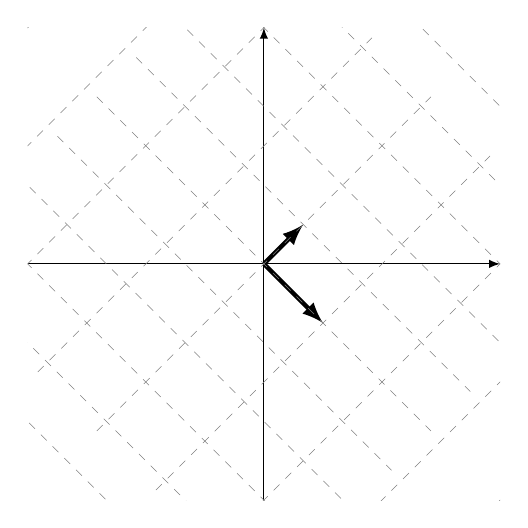
\begin{tikzpicture}
	\clip (-3,-3) rectangle (3cm,3cm);
    		\coordinate (Origin)   at (0,0);
    		\coordinate (XAxisMin) at (-3,0);
    		\coordinate (XAxisMax) at (3,0);
    		\coordinate (YAxisMin) at (0,-3);
    		\coordinate (YAxisMax) at (0,3);
    		\draw [thin,-latex] (XAxisMin) -- (XAxisMax);
    		\draw [thin,-latex] (YAxisMin) -- (YAxisMax);
		
		\coordinate (VecOne) at (0.5,0.5);
		\coordinate (VecTwo) at (0.75,-0.75);
    		\draw [ultra thick,-latex,black] (Origin)
        			-- (VecOne) node [above left] {};
    		\draw [ultra thick,-latex,black] (Origin)
        			-- (VecTwo) node [below right] {};
			
    		\pgftransformcm{0.707107}{-0.707107}{0.707107}{0.707107}{\pgfpoint{0cm}{0cm}}	
		\foreach \x in {-5,...,5}	
    		\draw[style=help lines,dashed] ({1.0606*\x},{-3}) -- ({1.0606*\x},{3});
		\foreach \y in {-5,...,5}
    		\draw[style=help lines,dashed] ({-3},{0.7071*\y}) -- ({3},{0.7071*\y});
	\end{tikzpicture}
  	\caption{The lattice for $\Z[\sqrt{2}]$ generated by $\langle 1,1 \rangle$ and $\langle \sqrt{2}, -\sqrt{2}\rangle$. \label{fig:lattice}}
	\end{figure} \xqed \pskip
\end{ex}


This last example is not an aberration.


\begin{prop}
Under the inclusion $\iota: K \hra K_\R$, the image $\iota(\O_K)$ is a discrete subgroup of the $\R$-vector space $K_\R$; that is, all its points $\iota(\O_K) \subseteq K_\R$ are isolated. 
\end{prop}

\pf Take $r>0$. It suffices to show there are only finitely many $\alpha \in \O_K$ with $|\sigma(\alpha)| \leq r$ for all $\sigma: K \hra \C$. Suppose $\alpha \in \O_K$ has this property. Then as $\alpha \in \O_K$,
	\[
	\prod_\sigma \big(x - \sigma(\alpha) \big)= p_\alpha(x)^{[K \colon \Q(\alpha)]} \in \Z[x].
	\]
By the assumption that $|\sigma(\alpha)| \leq r$, the coefficients of the polynomial on the left are bounded in terms of $r$ and $n$. Because of this and the fact that $\Z \subseteq \R$ is discrete, there are only finitely many possibilities for $\prod_\sigma (x - \sigma(\alpha))$. Hence, there are only finitely many such $\alpha$. \qed \\


While the next proposition is not directly related to the topics at hand, it will be useful later.


\begin{prop}\label{prop:zbasis}
Let $H$ be a discrete subgroup of $\R^n$. Then $H$ is a free $\Z$-module of rank at most $n$, and any $\Z$-basis of $H$ is linearly independent over $\R$. 
\end{prop}

\pf Let $V:= \Span_\R H$. Choose a basis for $V$ in $H$. We may assume $\Z^r \subseteq H \subseteq \R^r$, where $r= \dim_\R V \leq n$. Replacing $\R^n$ by $V$ if necessary, we may assume $\Z^n \subseteq H \subseteq \R^n$. Now every coset of $H/\Z^n$ has a representative with $(a_1, \ldots, a_n) \in \R^n$ with $0 \leq a_i<1$ (simply by rounding down each component and subtracting off a vector consisting of these numbers). Because $H$ is discrete, there are only finitely many such representatives. Hence, the quotient is finite. Set $m:= \#(H/\Z^n)$. Multiplying any element of $H/\Z^n$ by $m$ must give the identity coset, so multiplying any element of $H$ by $m$ lands in $\Z^n$. So $\Z^n \subseteq H \subseteq \frac{1}{m} \Z^n$. Therefore, $H$ must be free of rank $n$ as a $\Z$-module, i.e $H \cong \Z^n$. \qed \pskip


We can then obtain one of our long term goals, describing $(\O_K,+)$.


\begin{prop} \label{prop:ringintabelian}
Let $K/\Q$ be a number field of degree $n$. Then $\O_K \cong \Z^n$ as an additive abelian group.
\end{prop}

\pf By Proposition~\ref{prop:zbasis}, we know that $\O_K \cong \iota(\O_K) \subseteq K_\R \cong \R^n$. Therefore, $\O_K \cong \Z^r$, where $r \leq n$. Now take a basis $\{ x_1, \ldots, x_n \}$ of $K$ over $\Q$. After multiplication by some integer $m \geq 1$, i.e. clearing denominators as in Proposition~\ref{prop:power_push} (this does not affect linear independence), we may assume that $x_i \in \O_K$. Then $x_1, \ldots, x_n$ are linearly independent elements in $(\O_K, +)$. Therefore, $r \geq n$. But then we must have $r= n$. Hence, $\O_K \cong \Z^n$ as an additive abelian group. \qed \pskip


In general, how does one compute $\O_K$? We know how to compute $\O_K$ for quadratic extensions but not for a general number field $K$. We will introduce a `good guess' for the ring of integers (this will be what is called an order) and then correct this guess into the correct $\O_K$. For instance, if $K= \Q(\sqrt[3]{2})$, one would `guess' $\O_K \stackrel{?}{=} \Z[\sqrt[3]{2}]$. The theory of discriminants will allow us to check and adjust our guess, allowing us to work our way to the true ring of integers. 


\begin{dfn}[Order]
Let $K$ be a number field. An order of $K$ is a subring $R \subseteq K$ that is isomorphic as an additive group to $\Z^n$, where $n= [K \colon \Q]$. 
\end{dfn}


\begin{ex}
If $K= \Q(\sqrt[3]{2})$, then $\Z[\sqrt[3]{2}]$ is an order of $K$. \xqed \pskip
\end{ex}


\begin{ex}
By Proposition~\ref{prop:ringintabelian}, $\O_K$ is always an order of $K$. \xqed \pskip
\end{ex}


Indeed, $\O_K$ is the maximal order of $K$. One can define $\O_K$ to be the maximal order of $K$. However, it does take a bit of work to then show it is equivalent to our definition. 


\begin{lem} \label{lem:max_order}
For any order $R \subseteq K$, $R \subseteq \O_K$, i.e. $\O_K$ is the maximal order of $K$.
\end{lem}

\pf Take $\alpha \in R$. Then $\alpha R \subseteq R$. Note that $R$ is an order, i.e. a finitely generated $\Z$-submodule of $K$. But then by Propostion~\ref{prop:algint}, we know that $\alpha \in \O_K$. \qed \pskip


\begin{rem}
It is important to emphasize that although for any order $R \subseteq K$, $R \cong \O_K$ as additive abelian groups. However, Lemma~\ref{lem:max_order} shows that $R \subseteq \O_K$ as subrings of $K$. 
\end{rem}



% -------------------
% Discriminants
% -------------------
\subsection{Discriminants}

It is routine to verify that $\Tr{K/\Q}$ is a symmetric (non-degenerate) $\Q$-bilinear pairing on $K$:
	\begin{center}
	\begin{tikzcd}
	\langle \;,\; \rangle \arrow{r} & \Q \\[-3ex]
	(\alpha,\beta) \arrow[mapsto]{r} & \Tr{K/\Q}(\alpha\beta)
	\end{tikzcd}
	\end{center}
	
By Corollary~\ref{cor:mult}, $(\alpha,\beta) \mapsto \Tr{K/\Q}(\alpha \beta) \in \Z$ so that $\langle \;,\;\rangle: R \times R \to \Z$ for any order $R$. This induces a pairing on $K \otimes_\Q \R \cong K_\R$ and gives it a Euclidean structure, i.e. a standard inner product on $\R^n$. Fix a basis $\{ x_1, \ldots, x_r \}$ of $R$ as a $\Z$-module, and take $\alpha, \beta \in R$, writing them as
	\[
	\begin{split}
	\alpha&= \sum_{i=1}^r a_i x_i \\
	\beta&= \sum_{i=1}^r b_i x_i,
	\end{split}
	\]
where $a_i, b_i \in \Z$. Expanding the product and using the linearity of $\Tr{K/\Q}$, we have
	\[
	\Tr{K/\Q}(\alpha\beta)= \sum_{i,j} a_i \Tr{K/\Q}(x_ix_j)b_j= (a_1,\ldots,a_n) 
	\begin{pmatrix}
	\Tr{K/\Q}(x_1x_1) & \cdots & \Tr{K/\Q}(x_1x_r) \\
	\vdots & \ddots & \vdots \\
	\Tr{K/\Q}(x_rx_1) & \cdots & \Tr{K/\Q}(x_rx_r)
	\end{pmatrix}
	\begin{pmatrix}
	b_1 \\ \vdots \\ b_r
	\end{pmatrix}
	\]
This matrix will be our next object of study and is worthy of a name:

 
\begin{dfn}[Discriminant]
The discriminant of an $n$-tuple $(x_1, \ldots, x_n) \in \O_K^n$ is
	\[
	\disc(x_1,\ldots,x_n):= \det\left( \Tr{K/\Q}(x_ix_j) \right)_{i,j}
	\]
\end{dfn}


Note that the discriminant takes values in $\Z$ because $\Tr{K/\Q}$ takes values in $\Q$. But how does the discriminant depend on the choice of basis for $\O_K$? If one chose another basis of $R$, say $\{ y_1, \ldots, y_n \}$, write
	\[
	y_i= \sum_{j=1}^r B_{ij} x_j
	\]
for some $B_{i,j} \in \Z$. Define the matrix $B:= (B_{i,j})_{i,j}$. The matrix $B$ is symmetric and invertible, i.e. $B \in \GL_n(\Z)$. It is routine to verify that
	\[
	\left( \Tr{K/\Q}(y_iy_j) \right)_{ij}= B \left( \Tr{K/\Q}(x_ix_j) \right)_{ij} B^T.
	\]
Then taking determinants and using the fact that $\det M= \det M^T$, we have
	\[
	\disc(y_1, \ldots, y_n)= \det(B)^2 \disc(x_1, \ldots, x_n).
	\]
Because $B \in \GL(\Z)$, we must have $\det(B)= \pm 1$. Therefore, the discriminant is independent of the choice of basis. This proves the following proposition:


\begin{prop}
The discriminant of an $n$-tuple $(x_1, \ldots, x_n) \in \O_K^n$ is independent of the choice of basis for $\O_K$.
\end{prop}


\begin{dfn}[Discriminant of an Order]
The discriminant of an order $R$ is $\disc(R):= \disc(x_1, \ldots, x_n)$, where $\{ x_1, \ldots, x_n \}$ is a basis of $R$.
\end{dfn}


We can now make our previous `guess-and-check' notion for calculating $\O_K$ a bit more precise. As we shall show, for an order $R \subseteq \O_K$, $\disc(R)= \disc(\O_K) [\O_K \colon R]^2$, c.f. Lemma~\ref{lem:disc_ordersq}. Then to find $\O_K$, we have the following procedure: \pskip


\noindent{\bfseries Computing $\O_K$}
	\begin{enumerate}[1.]
	\item Guess an order $R$.
	\item Compute $\disc(R)$, which gives a finite number of possibilities for $[\O_K \colon R]$.
	\item Observe $R \subseteq \O_K \subseteq \frac{1}{m} R$. Find representatives for the cosets and determine which are algebraic integers. 
	\end{enumerate} \pskip


As a final remark before relating the discriminants of orders, we shall show that the discriminant is always nonzero which essentially follows because the pairing $\langle \;,\; \rangle$ is non-degenerate.


\begin{prop}
For an order $R \subseteq K$, $\disc(R) \neq 0$.
\end{prop}

\pf Suppose $0 \neq \alpha \in R$. We know $\Tr{K/\Q}(\alpha\alpha^{-1})= [K \colon \Q] \neq 0$ so that there is some $m \geq 1$ such that $m \alpha^{-1} \in R$. Then $\langle \alpha, \beta \rangle= m [K \colon \Q] \neq 0$ because $\langle \;,\; \rangle$ is non-degenerate. \qed \pskip


\begin{dfn}[Discriminant of a Number Field]
If $K$ is a number field, then we define the discriminant of $K$ to be $\disc(K):= \disc(\O_K)$. 
\end{dfn}


\begin{rem}
There are many notations for what we have denoted as $\disc(K)$: $d_K, D_K, \Delta_K, \ldots$.
\end{rem}


Before we prove a useful lemma relating $\disc(R)$ and $\disc(\O_K)$, we shall remind the reader of Smith Normal Form.


\begin{thm}[Smith Normal Form]
Let $B \in M_n(\Z)$ be of rank $r$. There exists matrices $P, Q \in \GL(\Z)$ such that
	\[
	PBQ=
	\begin{pmatrix}
	 d_1 &  &  &  &  & \\ 
	 &  \ddots &  &  &  & \\ 
	 &  &  d_r &  &  & \\ 
	 &  &  & 0 &  & \\ 
	 &  &  &  & \ddots & \\ 
	 &  &  &  &  & 0
	\end{pmatrix}
	\]
where $d_i \geq 1$ and $d_i \mid d_{i+1}$. 
\end{thm}


\begin{rem}
One only need the entries of the matrix be in a PID and the matrix need not be square. One defines $d_i= \div_i(A) / \div_{i-1}(A)$, where $\div_i$ is the $i$th determinant divisor, i.e. the gcd of all the $i \times i$ minors of $A$ and $d_0(A):= 1$. 
\end{rem}


\noindent {\bfseries Exercise:} Prove the classification of finitely generated abelian groups using the Smith Normal Form. \\


\begin{lem} \label{lem:disc_ordersq}
Let $R \subseteq K$ be an order. Then $\disc(R)= \disc(\O_K) [\O_K \colon R]^2$. 
\end{lem}

\pf Write $\O_K= \Z x_1 \oplus \cdots \oplus \Z x_n$ and let $R \subseteq \O_K$ be an order. Write $R= \Z y_1 \oplus \cdots \oplus \Z y_n$. For each of the $y_i$'s, write
	\[
	y_i \sum_{j=1}^n B_{ij} x_i.
	\]
Define $B:= (B_{i,j})_{i,j}$. We know that $B \in \GL_n(\Z)$. Observe that $[\O_K \colon R] = [\Z^n \colon B(\Z^n)]$. By some previous remarks,
	\[
	\disc(y_1, \ldots, y_n)= \det(B)^2 \disc(x_1, \ldots, x_n)= \det(B)^2 \disc(\O_K).
	\]
Therefore, $\disc(R)= \det(B)^2 \disc(\O_K)$. It remains to show that $\det(B)= \pm [\O_K \colon R]$. 

Using the Smith Normal Form, there are invertible integer matrices $P, Q$ so that $PBQ$ is a diagonal matrix. But then $\det(P), \det(Q) \in \{\pm 1\}$. But then $P,Q$ do not change $[\Z^n \colon B(\Z^n)]$ or $\pm\det(B)$. So without loss of generality, we may assume that $B$ is of the form
	\[
	B= \begin{pmatrix} d_1 & & \\ & \ddots & \\ & & d_n \end{pmatrix}
	\]
with $d_i \geq 1$ and $\det B \neq 0$. Now $\det(B)= d_1 d_2 \cdots d_n$. Therefore,
	\[
	B(\Z^n)= d_1 \Z \times \cdots \times d_n \Z
	\]
and
	\[
	\Z^n/B(\Z^n) \cong \Z/d_1\Z \times \cdots \times \Z/d_n\Z,
	\]
which has cardinality $d_1 \cdots d_n$, as desired. \qed \pskip


\begin{ex}
Let $K= \Q(\sqrt{d})$, where $d \neq 1$ is a squarefree integer. Now $R= \Z[\sqrt{d}]= \Z + \Z \sqrt{d}$ is an order of $K$. Furthermore,
	\[
	\begin{split}
	\disc(R)&= \disc(1,\sqrt{d}) \\
	&= \det \begin{pmatrix}
	\Tr{K/\Q}(1 \cdot 1) & \Tr{K/\Q}(1 \cdot \sqrt{d}) \\
	\Tr{K/\Q}(\sqrt{d} \cdot 1) & \Tr{K/\Q}(\sqrt{d} \cdot \sqrt{d})
	\end{pmatrix} \\
	&= \det \begin{pmatrix} 2 & 0 \\ 0 & 2d \end{pmatrix} \\
	&= 4d.
	\end{split}
	\]
So $4d= \disc(R)= \disc(\O_K) [\O_K \colon R]^2$. Because $d$ is squarefree, this implies that $[\O_K \colon R] \in \{ 1, 2 \}$; that is, $\O_K= R$ or is index 2 larger, i.e.	
	\[
	R \subseteq \O_K \subseteq \dfrac{1}{2}\, R.
	\]
Now $R / \frac{1}{2}R$ has coset representatives $1, \frac{1}{2}, \frac{\sqrt{d}}{2}$, and $\frac{1 + \sqrt{d}}{2}$. One need only check which of these are algebraic integers. It is routine to check that 1 is an algebraic integer, $\frac{1}{2}, \frac{\sqrt{d}}{2}$ are not algebraic integers, and $\frac{1 + \sqrt{d}}{2}$ is sometimes an algebraic integer (if and only if $d \equiv 1 \mod 4$). Therefore,
	\[
	\begin{split}
	\O_K&=
	\begin{cases}
	\Z[\sqrt{d}], & \text{if } d \not\equiv 1 \mod 4 \\ \\
	\Z\left[ \dfrac{1 + \sqrt{d}}{2} \right], & \text{if } d \equiv 1 \mod 4
	\end{cases} \\ \\
	\disc(\O_K)&=
	\begin{cases}
	4d, & \text{if } d \not\equiv 1 \mod 4 \\
	d, & \text{if } d \equiv 1 \mod 4.
	\end{cases}
	\end{split}
	\] \xqed \pskip
\end{ex}


\begin{rem}
The discriminant of $\O_K$ determines a degree 2 extension $K/\Q$ up to isomorphism. Later, we shall see that there are only finitely many number fields of any degree with a given discriminant. 
\end{rem}


\begin{lem} \label{lem:embeddisc}
Let $\sigma_1, \ldots, \sigma_n: K \hra \C$ be the complex embeddings of $K$ into $\C$. Then for $x_1, \ldots, x_n \in \O_K$,
	\[
	\disc(x_1, \ldots, x_n)= \bigg( \det \big(\sigma_i(x_j) \big)_{i,j} \bigg)^2= \left[ \det 
	\begin{pmatrix}
	\sigma_1(x_1) & \cdots & \sigma_1(x_n) \\
	\vdots & \ddots & \vdots \\
	\sigma_n(x_1) & \cdots & \sigma_n(x_n)
	\end{pmatrix} \right]^2
	\]
\end{lem}

\pf Recall $\Tr{K/\Q}(x)= \sum_{i=1}^n \sigma_i(x)$. Let $A:= (\sigma_i(x_j))_{i,j}$. Then we have
	\[
	\begin{split}
	\disc(x_1, \ldots, x_n)&= \det \bigg( \Tr{K/\Q}(x_ix_j) \bigg)_{i,j} \\
	&=\det \left( \sum_{k=1}^n \sigma_k(x_i) \sigma_k(x_j) \right) \\
	&=\det \left( \sum_{k=1}^n \sigma_k(x_i x_j) \right) \\
	&= \det( A^TA) \\
	&= \left[ \det(A) \right]^2.
	\end{split}
	\] \qed \pskip


\begin{ex}
Let $K= \Q(\sqrt{d})$, where $d \neq 1$ is a squarefree integer. Consider $R= \Z[\sqrt{d}] \subseteq \Q(\sqrt{d})= K$. The two complex embeddings of $K$ into $\C$ are 
	\[
	\begin{split}
	\sigma_1(a + b\sqrt{d})&= a + b\sqrt{d} \\
	\sigma_2(a + b\sqrt{d})&= a - b\sqrt{d}
	\end{split}
	\]
Then by Lemma~\ref{lem:embeddisc}
	\[
	\begin{split}
	\disc R&= \disc(1,\sqrt{d}) \\
	&= \left[ \det \begin{pmatrix}
	\sigma_1(1) & \sigma_1(\sqrt{d}) \\
	\sigma_2(1) & \sigma_2(\sqrt{d})
	\end{pmatrix} \right]^2 \\
	&= \left[\det \begin{pmatrix}
	1 & \sqrt{d} \\
	1 & -\sqrt{d}
	\end{pmatrix} \right]^2 \\
	&= 4d
	\end{split}
	\] \xqed \pskip
\end{ex}


The term `discriminant' will already be familiar to the reader from the discriminant of a polynomial. 


\begin{dfn}[Discriminant of a Polynomial]
If $f(x) \in \Q[x]$ is a monic polynomial of degree $n \geq 1$, the discriminant of $f$ is
	\[
	\disc(f)= \prod_{1 \leq i<j \leq n} (\alpha_i - \alpha_j)^2
	\]
where $\alpha_1, \ldots, \alpha_n$ are the roots of $f$ in $\C$. 
\end{dfn}


It is worth noting that $\disc(f) \in \Q$ and if $f \in \Z[x]$ then $\disc(f) \in \Z$. Note also that if the polynomial is not monic, one can always divide by the leading coefficient and use the fact that if $\alpha \in \Q$, then $\disc(\alpha x)= \alpha^n \disc(x)$, where $n=[K:\Q]$. 


\begin{ex}
Here are some discriminants of several specific polynomials:
	\[
	\begin{split}
	\disc(x^2 + bx + c)&= b^2 - 4c \\
	\disc(x^3 + bx^2 + cx + d)&= b^2c^2 - 4c^3 - 4b^3d - 27d^2 + 18bcd \\
	\disc(x^3 + cx + d)&= -4c^3 - 27 d^2
	\end{split}
	\] \xqed \pskip
\end{ex}


We shall connect the discriminant of a number field with that of the discriminant of a polynomial. 


\begin{lem}\label{lem:discmin}
If $\alpha \in \O_K$ is such that $K=\Q(\alpha)$ (so that $\Z[\alpha]$ is an order of $K$), then $\disc(\Z[\alpha])= \disc(p_\alpha(x))$, where $p_\alpha(x)$ is the minimal polynomial of $\alpha$ over $\Q$. 
\end{lem}

\pf Let $\sigma_1,\ldots,\sigma_n: K \hra \C$ be the complex embeddings of $K$ into $\C$. The roots of $p_\alpha(x)$ are $\sigma_1(\alpha),\ldots,\sigma_n(\alpha)$. Write $\alpha_i= \sigma_i(\alpha)$. The order $\Z[\alpha]$ has a  integral $\Z$-basis $\{1,\alpha,\ldots,\alpha^{n-1}\}$. Therefore,
	\[
	\begin{split}
	\disc(\Z[\alpha])&= \disc(1,\alpha,\ldots,\alpha^{n-1}) \\
	&= \left( \det \begin{pmatrix}
	1 & \alpha_1 & \alpha_1^2 & \cdots & \alpha_1^{n-1} \\
	1 & \alpha_2 & \alpha_2^2 & \cdots & \alpha_2^{n-1} \\
	\vdots & \vdots & \vdots^2 & \ddots & \vdots \\
	1 & \alpha_n & \alpha_n^2 & \cdots & \alpha_n^{n-1} 
	\end{pmatrix} \right)^2 \\
	&= \left( \prod_{1 \leq i < j \leq n} (\alpha_j - \alpha_i) \right)^2 \\
	&= \disc(p_\alpha(x))
	\end{split}
	\] \qed \\


\begin{ex}
Let $K=\Q(\alpha)$, where $\alpha$ is a root of $f(x)=x^3+x+1$. Observe that $f(x)$ is irreducible and then $[K:\Q]=3$. Now $\Z[\alpha]$ is an order of $K$ with 
	\[
	\disc(\Z[\alpha])= \disc(f)= -4(1)^3 - 27(1)^2= -31.
	\]
But $\disc(\Z[\alpha])= \disc(\O_K) [\O_K \colon \Z[\alpha]]^2$. Since 31 is prime, we must have $[\O_K \colon \Z[\alpha]=1$ which implies that $\O_K=\Z[\alpha]$ and $\disc(K)= -31$. \xqed \pskip
\end{ex}


\begin{ex}
Let $K=\Q(\alpha)$, where $\alpha$ is a root of $f(x)= x^3-x^2-2x-8$. Consider the order $\Z[\alpha]$ of $K$. 
	\[
	\disc(\Z[\alpha])= \disc(f)= -2012= -2^2 \cdot 503.
	\]
Then $[\O_K \colon \Z[\alpha]] \in \{1,2\}$. Therefore,
	\[
	\Z[\alpha] \subseteq \O_K \subseteq \dfrac{1}{2} \, \Z[\alpha]
	\]
The group $\frac{1}{2}\Z[\alpha]/\Z[\alpha$ has coset representatives $\frac{a}{2} + \frac{b}{2} \alpha + \frac{c}{2} \alpha^2$, where $a,b,c \in \{0,1\}$. We need only check which of these eight elements are algebraic integers. Let $\theta:= \frac{\alpha + \alpha^2}{2}$. Now $K$ has $\Q$-basis $\{1,\alpha,\alpha^2\}$ and $\theta$ acts on this by
	\[
	\begin{split}
	\theta \cdot 1&= \frac{1}{2} \alpha + \frac{1}{2} \alpha^2 \\
	\theta \cdot \alpha&= 4+\alpha + 2\alpha^2 \\
	\theta \cdot \alpha^2&= 8 + 6\alpha +2\alpha^2
	\end{split}
	\]
Therefore, $\theta$ is a root of 
	\[
	\det\left(xI - 
	\begin{pmatrix}
	0 & 4 & 8 \\
	^1/_2 & 1 & 6 \\
	^1/_2 & 1 & 2 
	\end{pmatrix}
	\right)= x^3 - 3x^2 -10x - 8.
	\]
But then $\theta \in \O_K$. Therefore, $\O_K= \Z 1 \oplus \Z \alpha \oplus \Z\frac{\alpha+\alpha^2}{2}=\Z \oplus \Z \alpha \oplus \Z \theta$. Note that $\O_K \neq \Z[\beta]$ for any $\beta \in \O_K$ --- a result due to Dedekind. \xqed \pskip
\end{ex}


\begin{ex}
In the previous example, we saw that for $K=\Q(\alpha)$, where $\alpha$ is a root of $f(x)=x^3-x^2-2x-8$, $\O_K \neq \Z[\beta]$ for any $\beta \in \O_K$. This is not the only example. For example, if $K=\Q(\sqrt[3]{19})$, then $\O_K \neq \Z[\sqrt[3]{19}]$ but rather $\O_K=\Z+\Z\omega+ \Z \frac{1+\omega+\omega^2}{3}$, where $\omega=\sqrt[3]{19}$. \xqed \pskip
\end{ex}


We have seen how the discriminant relates to $\O_K$. We shall now see how the discriminant relates to the norm.


\begin{lem}\label{lem:discnorm}
Let $K=\Q(\alpha)$ be a number field, where $\alpha \in \O_K$. If $f \in \Z[x]$ is the minimal polynomial of $\alpha$ over $\Q$, then	
	\[
	\disc(\Z[\alpha])= \disc(f)= (-1)^{\frac{n(n-1)}{2}} \Nm{K/\Q}(f'(\alpha))
	\]
In particular, $\disc(\Z[\alpha]) \in \Q$. 
\end{lem}

\pf The first equality was Lemma~\ref{lem:discmin}. For the second equality, let $\sigma_1,\ldots,\sigma_n: K \hra \C$ be the complex embeddings of $K$ into $\C$. By rearranging terms,
	\[
	\begin{split}
	\disc f&= \prod_{1 \leq i < j \leq n} (\sigma_i(\alpha) - \sigma_j(\alpha))^2 \\
	&= (-1)^{\binom{n}{2}} \prod_j \prod_{i \neq j} (\sigma_j(\alpha) - \sigma_i(\alpha))
	\end{split}
	\]
However, we know $f=\prod_i (x - \sigma_i(\alpha))$. Using the product rule, this gives 
	\[
	f'= \sum_j \prod_{i \neq j} (x - \sigma_i(\alpha)).
	\]
But then $f'(\sigma_j(\alpha))= \prod_{i \neq j} (\sigma_j(\alpha) - \sigma_i(\alpha))$ since all but one term vanishes. Using this in the above along with the fact that the $\sigma_i$ fix $\Q$ (hence fix the coefficients of $f'$), we have
	\[
	\begin{split}
	(-1)^{\binom{n}{2}} \prod_j \prod_{i \neq j} (\sigma_j(\alpha) - \sigma_i(\alpha))&= (-1)^{\frac{n(n-1)}{2}} \prod_j f'(\sigma_j(\alpha)) \\
	&= (-1)^{\frac{n(n-1)}{2}} \prod_j \sigma_j(f'(\alpha)) \\
	&=  (-1)^{\frac{n(n-1)}{2}} \Nm{K/\Q}(f'(\alpha))
	\end{split}
	\] \qed \pskip


\begin{ex}[$p$th Cyclotomic Field]
Fix an odd prime $p$. Let $\zeta \neq 1$ be a $p$th root of unity, i.e. $\zeta^p=1$. Let $K=\Q(\zeta)$ be the $p$th cyclotomic field. Define
	\[
	f(x):= \dfrac{x^p-1}{x-1}= x^{p-1} + x^{p-2} + \cdots + x + 1 \in \Z[x]
	\]
Observe that $f(\zeta)=0$ and that $f$ is irreducible (examine $f(x+1)$, use Eisenstein's criterion, then invoke Gau\ss' lemma). In particular, $[K\colon \Q]=p-1$. Now what is $\O_K$. We have the `obvious guess' of the order $\Z[\zeta]$. We need to check this guess. We know $\disc(\Z[\zeta])= (-1)^{\frac{(p-1)(p-2)}{2}} \Nm{K/\Q}(f'(\zeta))$. But what is $f'(\zeta)$? We first calculate $f'(x)$, then evaluate at $\zeta$:
	\[
	\begin{split}
	(x-1)f(x)&= x^p - 1 \\
	f(x) + (x-1) f'(x)&= p x^{p-1} \\
	f'(\zeta)&= \dfrac{p \,\zeta^{p-1}}{\zeta-1}
	\end{split}
	\]
Note that $[K \colon \Q]= \phi(p)=p-1$ and $\zeta \in \O_K^\times$. Let $\sigma_1,\ldots,\sigma_n$ be the complex embeddings of $K$ into $\C$. Then noting that $p-1$ is even and $f(x)=\prod_i (x-\sigma_i(\zeta))$, we have
	\[
	\begin{split}
	\Nm{K/\Q}(\zeta-1)&= (-1)^{p-1} \Nm{K/\Q}(1-\zeta) \\
	&=\Nm{K/\Q}(1-\zeta) \\
	&=\prod_{\sigma: K \hra \C} \sigma(1-\zeta) \\
	&= \prod_{\sigma: K \hra \C} (1-\sigma(\zeta)) \\
	&= f(1) \\
	&= 1 + 1 + \cdots + 1 \\
	&= p
	\end{split}
	\]
We know $(\zeta -1) f'(\zeta) = p \zeta^{p-1}$. Taking norms gives
	\[
	\begin{split}
	\Nm{K/\Q}(\zeta-1) \Nm{K/\Q}(f'(\zeta))&= \Nm{K/\Q}(p) \Nm{K/\Q}(\zeta)^{p-1} \\
	\Nm{K/\Q}(\zeta-1) \Nm{K/\Q}(f'(\zeta))&= p^{p-1} (\pm 1)^{p-1} \\
	p \Nm{K/\Q}(f'(\zeta))&= p^{p-1}
	\end{split}
	\]
Therefore, $\disc(\Z[\zeta])= (-1)^{\frac{(p-1)(p-2)}{2}} p^{p-2}=(-1)^{\frac{p-1}{2}} p^{p-2}$, since $p$ is odd. Note that we lose nothing by assuming that $p$ is odd: if $p=2$, then $\Q(\zeta)=\Q$. Then if $\Z[\zeta] \subsetneq \O_K$, it must be that $[\O_K \colon \Z[\zeta]]=p^e$ for some $e \geq 1$. After possibly multiplying by a power of $p$, we know there is a $\alpha \in \O_K$ such that $\alpha \notin \Z[\zeta]$ and $p\alpha \in \Z[\zeta]$. We know $\Z[\zeta]= \Z[\zeta-1]$. Then $\alpha$ can be written
	\[
	\alpha = \dfrac{a_0}{p} + \dfrac{a_1}{p} (\zeta-1) + \cdots + \dfrac{a_{p-2}}{p} (\zeta-1)^{p-2},
	\]
where $a_i \in \Z$ with not all $a_i$ divisible by $p$. Subtracting multiples of $p$ from those terms divisible by $p$, we may assume $a_i$ is not divisible by $p$ for $0 \leq i \leq p-2$. Hence, we can write
	\[
	\alpha = \dfrac{a_i}{p} (\zeta-1)^i + \cdots + \dfrac{a_{p-2}}{p} (\zeta-1)^{p-2},
	\]
where $p \nmid a_i$. Multiplying by $\frac{p}{(\zeta-1)^{i+1}}$, we have
	\[
	\dfrac{p\alpha}{(\zeta-1)^{i+1}} = \dfrac{a_1}{\zeta-1} + \underbrace{a_{i+1} + a_{i+2}(\zeta-1) + \cdots + a_{p-2}(\zeta-1)^{p-2-(i+1)}}_{\in\, \Z[\zeta]}
	\]
Now $\Nm{K/\Q}(\frac{a_i}{\zeta-1})= \frac{a_i^{p-1}}{p} \notin \Z$ as $p \nmid a_i$. But then $\frac{a_i}{\zeta-1} \notin \O_K$. But then using the above equality, this shows $\frac{p}{(\zeta-1)^{i+1}} \alpha \notin \O_K$. But as $\alpha \in \O_K$, this shows $\frac{p}{(\zeta-1)^{i+1}} \notin \O_K$. Therefore, $\frac{p}{(\zeta-1)^{i+1}} \notin \Z[\zeta]$. On the other hand,
	\[
	\begin{split}
	p&= \Nm{K/\Q}(\zeta-1) \\
	&= \prod_{\sigma} (\sigma(\zeta)-1) \\
	&=\prod_{i=1}^{p-1} (\zeta^i -1)
	\end{split}
	\]
Using the fact that $\zeta^i-1=(\zeta-1)(1+\zeta+\cdots+\zeta^{i-1})$, this shows that $(\zeta-1)^{p-1} \mid p$ in $\Z[\zeta]$. But as $i+1 \leq p-1$, this contradicts the fact that $\frac{p}{(\zeta-1)^{i+1}} \notin \Z[\zeta]$. Therefore, we know 
	\[
	\begin{split}
	\O_K&=\Z[\zeta] \\
	\disc \O_K&= (-1)^{\frac{p-1}{2}} p^{p-2}
	\end{split}
	\]
Note that $\frac{p}{(\zeta-1)^{p-1}} \in \Z[\zeta]$ and $\Nm{K/\Q}(\frac{p}{(\zeta-1)^{p-1}})= \frac{p^{p-1}}{p^{p-1}}=1$ so that $p=u(\zeta-1)^{p-1}$ for some $u \in \Z[\zeta]^\times$. \xqed \pskip
\end{ex}


\begin{rem}
Choose $m \geq 1$ and let $\zeta_m$ be the primitive $m$th root of unity. Then $\O_K=\Z[\zeta_m]$ and $\disc \O_K \mid m^{\phi(m)}$. 
\end{rem}

